\chapter{Implementation}
\label{chap:implementation}

% What is this chapter about?

\section{API}
\label{sec:apiImpl}
% How was the API implemented? Which frameworks? How can we use the same model to create different json representation for the client?  What was the thoughts behind the architecture used in API? Challanges? What could have been implemented better? What is left? 
% Need to define what REST stands for (remember reference)
\subsection{RESTful Architecture}
The back-end of the project has been implemented in a RESTful architecture, as this was one of the system requirements from the product owner. It was required that the back-end API would be robust, easy to use, efficient and restful in that way that it complies with the representational state transfer architectural style designed. \newline 
The idea behind using a RESTful approach for implementing the web service for the project is the fact that it separates the concerns between client and server. Based on that, the front-end or the clients are not concerned about the data storage which is a operation that remains internal to the server resulting in portability of client code. The server on the other hand is not concerned either with the user interface that will represent the processed information, nor the user state, hence the term stateless \cite{RESTRef}. Based on this design and also based on the system requirements to develop an API, the system architecture became a rather convenient task. The architectural properties of REST are achieved by applying specific interaction constraints to all the components and data elements. The constraints applied in this architectural design include: Client-Server uniform interface, Stateless communication, Cachable responses, Layered System and Code on Demand \cite{RESTRef}. It is important that any service that is implemented using the REST architecture, it has to conform and not violate the architectural constraints, otherwise it is not considered RESTful anymore. The communication between client and server is possible through sending HTTP request to the  resources that reside in the server side which also have defined HTTP Methods that carry out a specific action/operation in the back end. These methods derive from HTTP verbs (e.g. GET, POST, PUT, DELETE), and each of those are called using the URI of a resource, for example '/api/categories/1', where a DELETE call on that URI would carry an operation to delete a category with the ID 1.

The concept "stateless" plays an important role in REST. Here it is implied that the client-server communication is further constrained by not storing any client contexts on the server between requests that are initiated. Due to this, the system has been implemented in such a way that each request initiated from the client side will contain all the necessary information for the server to service the request, perform the necessary operations on it. The server might create and maintain a persistent state for a period of time for authentication purposes if necessary, but the session state is held in the client. 

Another important feature of the REST architectural style is its emphasis an uniform interface between components. To achieve an uniform interface there are some architectural constraints placed on the components that have to be satisfied. These constraints are defined as: identification of resource, manipulation of resources through representations (Hence representational state transfer), self-descriptive messages of the responses and hypermedia as the engine of the application state. One side-effect from having a system following the REST architecture is that it is very easily scalable as the back end does not hold the state of the current user (except on data level). This architecture is being widely used by corporate companies and even though it may be seen as quite strict and isolating in some extent, it provides a standardized, open and well-defined interface for application and infrastructure services.

\subsection{Implementation of the API}
Java programming language has been used to implement the back-end of the API as this was a familiar programming language for many of the team members. Hibernate was used as ORM (Object Relational Mapping). We used Glassfish as an application server which allows developers to create applications that are portable, scalable and that integrate with legacy technologies. 

\begin{figure}[h]
  \centering
  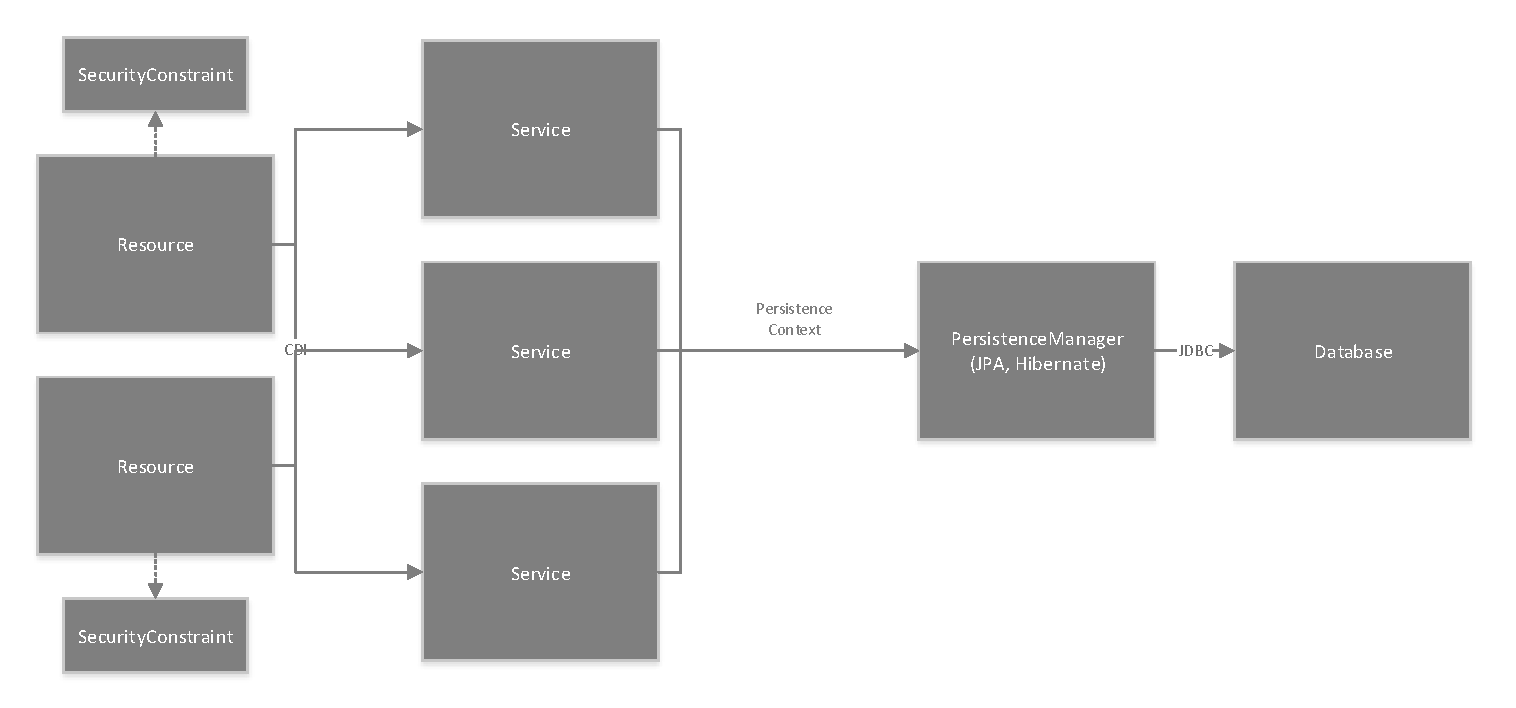
\includegraphics[width=\linewidth]{figures/API_architecture.pdf}
  \caption[API architecture.]{Overview of the API architecture.}
  \label{fig:apiArchitecture}
\end{figure}

The whole API is separated into four layers: Resources, Services, Model and Security Layer. The \textbf{Resource} layer includes all the classes that the client communicates with by sending requests to and receiving responses from in a JSON format. The system is not limited to respond with JSON format only, it is also possible to specify the response type as XML format. Inside the resource classes we have defined the necessary HTTP methods as mentioned in the previous section where each of them does a specific operation on the API such as retrieving object data, creating new entries, modifying existing ones and deleting if necessary. All of these operation are carried out through the GET, POST, PUT and DELETE HTTP methods. There are also sub-resources which extend from a main resource that carry out additional operations on a specific context. 
The uniform resource locators developed in this projects attempts to follow the REST constraints while the URIs to different resources attempts to follow the same conventions that Google has on their URIs. 
Almost every resource on the API which operates upon a model using a specific service has initially the main operations for retrieving a list or the object itself, modifying the state of the object, creating a new instance and persisting it into the application server and the Database, and finally removing the objects instance from the database. Besides these main operations such as user and token management, there are also additional resource methods that carry out other operations such as making API calls directly to Google to retrieve information. 
Besides this, together with the resources, Request Beans were used as objects that specify the information to be sent from the client (all the necessary parameters defined by its name and value) that the resource requires to carry out an operation. Usually these request beans are used when initiating a POST request to the API when creating new instances of objects. Another important thing about the request beans is its relation with JSON data, as it acts as a JSON object that holds the information the client has to send to the server. These objects have been annotated with XmlRootElement and XmlElement annotations so that it can be represented as such when posting and getting information data in either JSON or XML format respectively.

\textbf{Services} on the other hand serves acts as a bridge that the resources can use to communicate with the data layer by retrieving information, storing new ones, etc. All the service classes are stateless session beans, where a session bean is a type of enterprise bean which is normally used to do independent operations as per its name does not have any associated client state, but it may preserve its instance state. From this we benefit by using the dependency injection \cite{DependencyInjectionRef} design pattern into the resource objects. The service classes have been injected into the resource classes, where then the service is made part of the resources state. Passing the service to the resource object, rather than allowing it to find or build the service is a fundamental requirement of the pattern which helps implementing and maintaining inversion of control. This design pattern plays an important role when it comes to implementing independent layers from each other. Because injecting the services into the resource classes without actually creating new instances of it helps isolate the client (which in this case are the resource classes that access them) from the impact of design changes and defects that may occur. This design pattern promotes re-usability, testability and maintainability of code.
All service classes use a persistence context of the Entity Manager to communicate with the database. A persistence context is a set of entity instances in which for any persistent entity identity there is a unique entity instance. In our case, entities are considered all the defined model classes that are used to precess and interpret data within the API. Within the persistence context, the entity instances and their life-cycle are managed. The EntityManager API on the other hand is used to create and remove persistent entity instances, to find entity instances by their primary key, and to query over entities. All these operations are implemented inside methods of course, which are then used by the resources classes. The transactions carried out by the EntityManager and the persistence context are all atomic, meaning that all the transactions will try to be executed and if any failure occurs, all the changes will be rolled back so that the state of the database is maintained. Any occurring database violations are handled by the persistence context and will automatically fire exception which is further delegated to the resource classes which sends back the error message as a response to the client that a constraint has been violated and that the operation can not be carried out.

\textbf{Model} is the third layer of the API that is used for designing the model of all the objects whose information will be stored in the application layer and database. This models are mainly used to represent the data in a certain way that is understandable for the client and also suitable for the API itself (leading to a robust, stable, configurable, maintainable and reusable model). Using the Hibernate ORM saved us a lot of time not writing sql DDL queries because the framework made it possible to automatically converted the model java classes to database tables with all the attributes, data types, primary key, foreign key constraints and other relational database constraints as well. Inside the model class we have specified the relationships between two entities as either ManyToMany, OneToMany or ManyToOne as Java persistence annotations, where in the relational database it is represented as foreign key or as an extra table for many-to-many relationships. There are also cascade constraints applied to relationships which specifies that changes should propagate throughout the system. The side-effect of this is that the database gets easier to manage without any intervention from a developer.The default cascade type for most of the relationships is "remove" indicating that when a independent instance of an object is removed from the database, than all the corresponding dependent instances of the relation will be deleted respectively \cite{CascadeTypeRef}. It is worth mentioning that the model has been designed in such a way that it is used to represent the tables/entities from the database and also contains information on how the data should be represented to the client, for example as a JSON object.

The last layer in the API architecture is the \textbf{Security} layer. It consists of security filter that will make sure the user who is accessing the resources has the right to do so. There is one general filter called the Authentication Filter which checks if the user accessing the resources is authorized and its authorization token has not expired yet. When the user signs in using the Google credentials, the API generates an authorization token which has a period of time that is valid, but additionally a refresh token is also generated for the user which later on can be used to get a new valid authorization token from the API. Besides the authorization filter, there are other customized filters who extend the authorization filter. Before explaining how the customized filters works, it is important to note that most of the model types in this system are configured as user-specific. This means that when an instance of an object model is created, a relationship between that instance and the user who is registering it respectively is also created. This allows the customized filters to check if the resource being accessed from the logged user, tries to initiate operations on an instance object of a specific model if it is associated with that logged user or not. Otherwise, a HTTP 403 Forbidden error message will be sent back to the client in order to inform that it does not have sufficient permissions to access that resource. It has been made sure that every resource in our API is secured at least with the Authorization Filter, and for the resources that access user specific information, the customized filters are checked additionally. 

\subsection{Challenges}
%Noone new what we were ging to do
%me and martin had experiences with the frameworks
%Some of us had to learn AngularJS some had to further gain knowledge for programming in java
%Only one of the members knew how to write testing (and that only unit tasting)
%Developing RestFul api experience (one group member)
Several challenges were encountered from the first day of the development of the project. Initially, many of the team members were not familiar with the programming languages that were used to develop the API and the front end, therefor it took some time until all the group members were comfortable and could understand the code that was being written. Besides the fact that the work had been distributed throughout the members where some worked in the back end and some in the front end, still it was necessary that everyone understood all the different implementation parts of the project. The understanding complexity of the project was relatively high in the beginning even though the user stories that explained what the API should do and how it should operate, the team members were unable to grasp everything without doing further research on somewhat similar APIs. 

Writing unit tests and using Mockito \cite{mockitoRef} test framework was also one of the challenges where many of the group members had to learn from scratch as they did not have any experience within this field. Nevertheless, the team members that wrote tests on the API managed to understand how unit testings are implemented and how the Mockito framework is used in a relatively short period of time.

It was required to use JIRA powered by Attlasian as a Project Management tool for planning sprints, tracking the progress of the work, managing issues and bugs etc. Since JIRA is a relatively big project management tool, in the beginning it was very frustrating when trying to figure out and understand which functionalities were appropriate for our API project. Estimating working time to be spent on implementing functionalities during the sprints was also quite challenging. As a result, the time estimation for the first sprints were totally underestimated and the team members had to either drop some tasks and leave it to the next sprint or split it into sub tasks and re-estimate the time over again. It is worth mentioning that the team learned a lot from the time estimation concept, because it turned out that the last sprint was very well planned and the estimation was relatively similar to the actual work that had been done in the sprint.

It was mentioned earlier that in the Security Layer of the API, customized security filters had to be implemented from scratch because there was no standardized way on how to do it, or framework that was suitable for the security issues of this API. Because it was required that the implementation of the security layer had to be left at the end after the functional requirements of the API have been realized, it turned out to be very challenging as many changes had to be done in all the other layers such as the Resource and Model layers of the system. These changes and implementation at a later stage of the security constraints increased potential vulnerabilities in the system that might not have been covered.

\subsection{Further Improvements}
\label{sec:furtherImprovements}
%smaller sprints, git flow because team was not properly familiar with git
%deploy api as a microservice that is more convenient to deploy and set up
The security layer is one of the things that could have been improved without leaving any possible vulnerabilities in the system by planning from the beginning of the project rather than leaving it in the end. This is something that the team members learned from and hopefully wont occur in future projects. The velocity in each sprint may have been higher if the duration of the sprint would have been smaller than four weeks. Smaller sprints would make it possible to give better estimation on the work that needs to be done, and also motivate the team to work more regularly than in longer sprints. 
No branching feature from the Git version control system has been used during the development of the project. This was because some of the team members were not properly familiar with Git itself as a version control system.

Currently the API is not deployed as a micro-service, but is rather deployed as a web-application into an application server together with all the libraries and dependencies that the API uses in order to operate. Deploying it as a micro-service has a lot of benefits first and foremost because its easy to deploy (without setting up an application server), it is 
more lightweight as it allows modulation of the application server. Compared to the current deployment, utilizing the API as a microservice would make it possible to strip down the application server by not including many of the features that this project did not use. Micro-services are far more manageable compared to other architectures which are more monolithic in a way that everything is stored made available in one system, while micro-services are more separated and independent from each other.
\subsection{Remaining Work}
%Implementation of test in the front end
%Integration tests
%Performance analysis 
According to the user stories and the product owner requirements, the project is finished and ready to use. However, there are some other issues which have to be taken into consideration when building a project like this. Mostly, the remaining work that was left behind due to lack of time and which has to be done is regarding the testing part. In this project there is a complete working Unit testing in all the resources and services in the back end. The front end is lack of a testing part, mainly because of the time left but also because the product owner did not prioritize that part. There are a lot of different testing frameworks which can be applied in the front end e.g. Charma, Mocha, QUnit, etc. Writing the unit testing in front end from the beginning and as the project goes along it is quite challenging because the front end constantly faces changes, re-factoring, abstracting parts away, etc. 

In addition to the unit testing on both back end and front end, integration testing would also be another part which should have been developed, which is a logical extension of unit testing. This means that, two units which have been already tested, are combined into a component and the interface between them is tested \cite{Integ86:online}. This type of testing occurs after unit testing and before validation testing. Integration testing have to be applied in both parts of the project in order to verify functionality, performance and reliability requirements. This includes also verifying the implementation of individual components and their interconnection behavior when they are used together.
Performance analysis is anther task that has not been carried out during the project and which is an important process to be considered as remaining work. Due to lack of time and also prioritization of other processes the team was not able to test the performance of the API calls in the system. The project itself will not deal with large amount of data as it is only a different representation of analytics data provided by Google. Therefor critical performance analysis and improvements would not make a significant difference for the level of data analysis the system deals with.
\section{UI Prototype}
\label{sec:angularImpl}
% How was the UI implemented? Why is Angular so awesome? How does SPA work with an API and why is it a good idea to make an SPA instead of a PhP website?  
The User Interface (UI) was implemented using AngularJS, a JavaScript framework which is used to create single-page applications (SPA) \cite{Angul93:online}.
The goal of SPA is to provide a more smooth user experience, all the necessary code - HTML, CSS and JavaScript are loaded with single page load. When the user navigates trough the application, the entire application does not reload, only the required view is loaded. For example if the user wants to delete a web property, it is deleted from the variable holding the web property and the view is updated accordingly. Some of the benefits of using SPA include the separation of UI and data, the communication with the server is via JSON objects this allows both parts (backend and UI) to be developed and tested separately. It also makes it possible for developers with rather different background to work independently of each other.
Also SPA are easy to debug with built-in developer tools in a browser, as this enables monitoring of network operations, see the API calls, monitor what variables are passed to the functions, etc. \cite{What51:online}.

In the traditional way of creating web-applications, whenever CRUD operations (create, read, update, delete) is performed, the HTML page has to be reloaded in order to see the changes. 

The API calls are sent using \textdollar resource. Invoking a \textdollar resource object method immediately returns an empty reference (object or array, depending on whether \texttt{isArray} is set). Once the data is returned from the server, the callback function provided to the resource is executed accordingly \cite{Angul96online}.

\begin{figure}[h]
  \centering
  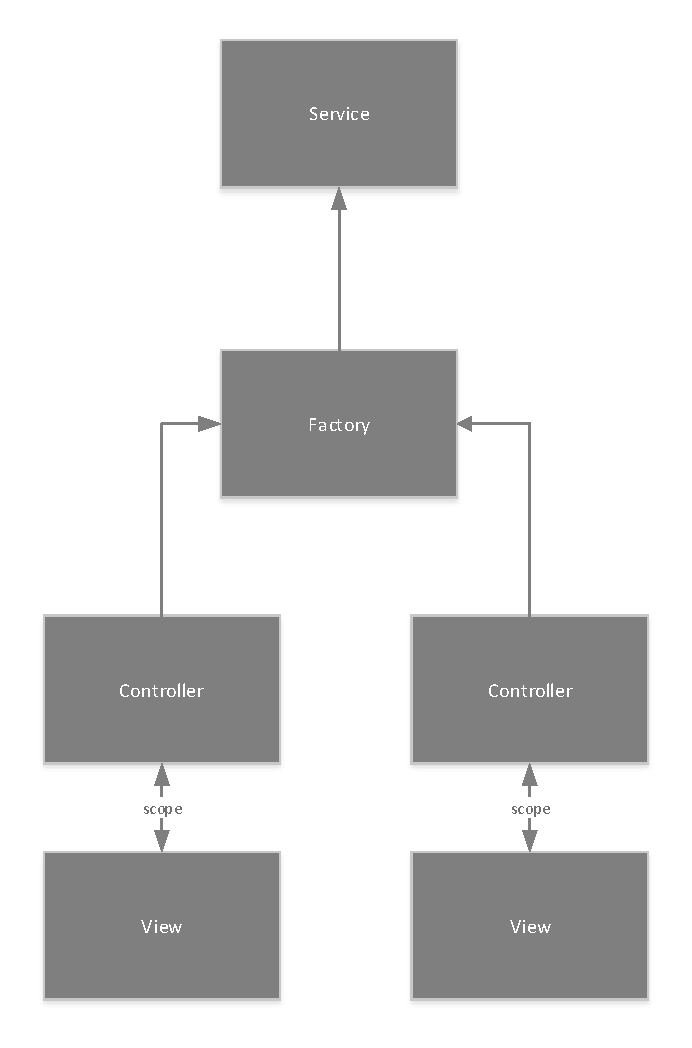
\includegraphics[width=.5\textwidth]{figures/AngularComponents.pdf}
  \caption[Angular components.]{Overview of the Angular components.}
  \label{fig:angularComponents}
\end{figure}

As shown in the Figure~\ref{fig:angularComponents}, the structure of the application is divided into controllers, factories, services and views: 

\begin{description}
\item[Controllers:] 
Controllers are responsible to take care the  interaction of the user with the view, assigning and updating the scope of a variable that holds the JSON response, defining conditions for success messages, etc. Each view has its own controller but can exist independently of a controller. A controller can also communicate with different factories.
For example when the function to delete Google Analytics account (\texttt{deleteGoogleAnalyticsAccount}) is called from the view (\texttt{GoogleAnalytics.html}), it passes the Google Analytics account ID to the controller, then the controller \texttt{GoogleAnalyticsController} is passing the ID to the factory \texttt{AccountFactory} and the variable is tailored according to the API call. Finally the variable is passed to the service (\texttt{AccountService}) where the DELETE request is performed. % Could mention how the callbacks works
The callbacks, success and error are called depending on the status code of the API call. An HTTP response status code between 200 and 299 is considered a success status \cite{Angul36:online}.


\item[Factories:] Factories are tailoring the JSON object that needs to be sent to the API call. 
When doing a POST request towards the API, the parameters that are injected in the URL and the body of the requested are set in the appropriate factory. \texttt{assignTagToWebsite} in \texttt{TagFactory} is an example of this, Google Analytics ID and web property ID should be passed in the URL while the name of the tag should be passed in the body of the POST request. % What URL? %mile: how should i call the url that the requests is sent to? You have to specify what the URL is, for example the URL for an API call.
Each factory has an appropriate service but also can communicate with different services.

\item[Services:] The API calls are defined here, the URL with the appropriate parameters for headers and default parameters when needed. All the calls return resource object. % Should mention that the URL is also defined in the services

For GET and DELETE requests the default parameters that are injected in the URL are defined here. % This also goes for all other HTTP verbs

\item[Views:] The view is what the user sees and interacts with the application. If the API call returns a JSON object that needs to be represented to the user, \texttt{ng-repeat} is used to display the needed information. If the API call does something in the background for example when adding all the webproperties from a Google analytics account in the current view only a success message is displayed to user that all web properties were added.
%The data from the API call is displayed in the view, since it is JSON ng-repeat is used to loop trough it and display the needed information. % The data from the API call is displayed in the view as it is available through the scope variable. It is possible to make API calls without displaying the returned data from the API (I believe this happens everal places in our case)
\end{description}

Grunt was used for building the application, starting the local server together with the app. 

JSHint was used for code quality checks. It checks for simple typos mistake, missing semicolon or potential bugs.

Bower was used to install packages and dependencies that were needed in the project such as Angular, Bootstrap etc.